\documentclass[handout]{beamer}

\usetheme{default}
\usecolortheme{default}

\title{The Waterfall Method}

\author{Lucas JACQUIN, Corentin MENGEL, Vincent ITALIANO, Antoine SCHUFFENECKER, Abdelhamid MOLTAZIM}

\begin{document}
\begin{frame}    
    
    \maketitle

\end{frame}

\begin{frame}
    \frametitle{Introduction and history}
\end{frame}

\begin{frame}
    \frametitle{Phases of waterfall project management}
    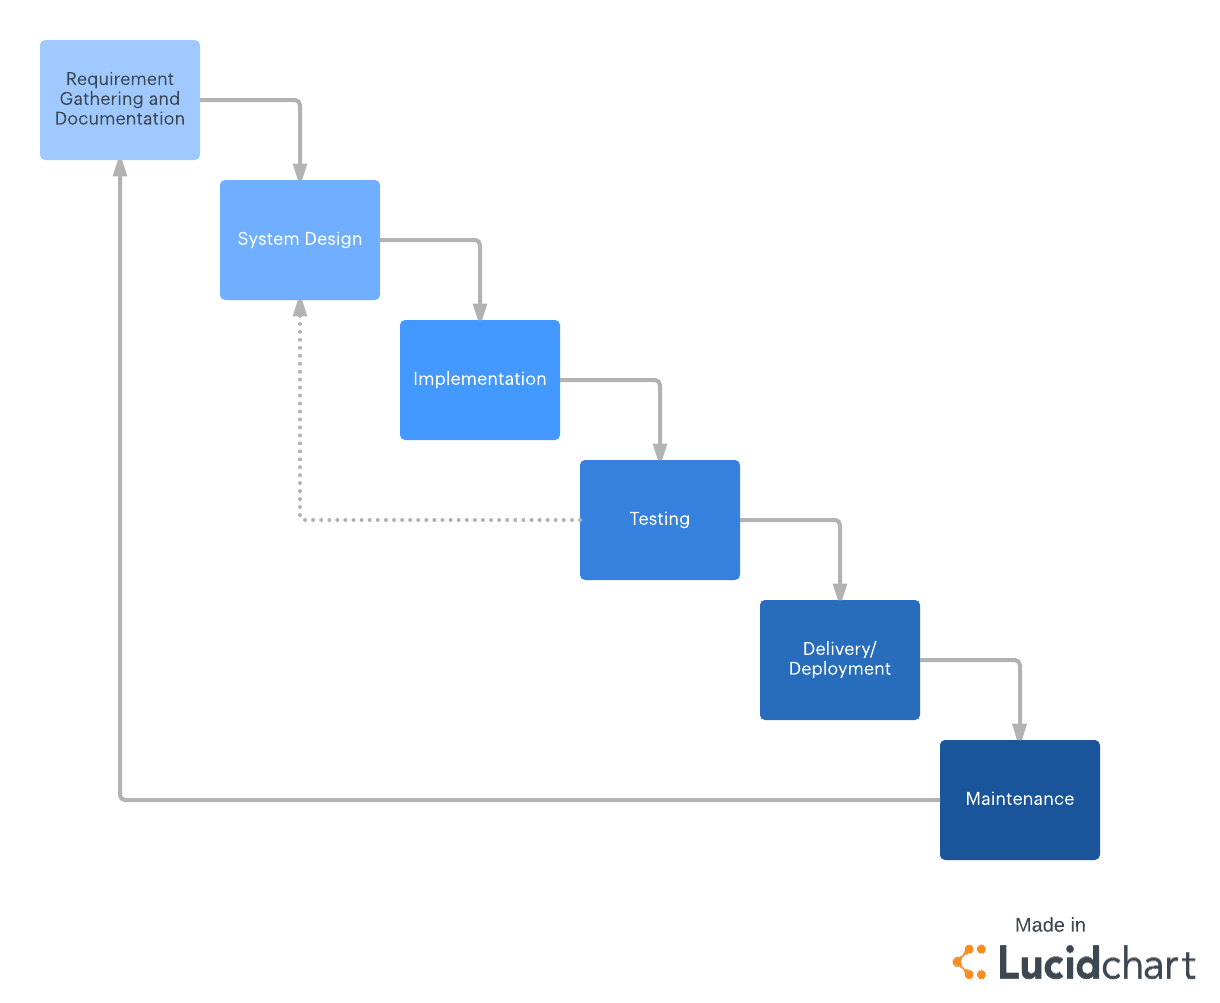
\includegraphics[scale=0.25]{Images/WaterfallDiagram.png}
\end{frame}

\begin{frame}
    \frametitle{Phases of waterfall project management}
    \begin{itemize}
        \setlength\itemsep{1em}
        \item Requirement gathering and documentation \pause
        \item System design \pause
        \item Implementation \pause
        \item Testing \pause
        \item Delivery/deployment \pause
        \item Maintenance
    \end{itemize}
\end{frame}


\nocite{*}
\begin{frame}
    \frametitle{Bibliography}

    \bibliographystyle{plain}
    \bibliography{waterfall}    

\end{frame}

\end{document}